\scanpage{86}
\mspage{85}
% slanted
\margin{\uline{NB} \unsure{Si on ne|Sans} \unsure{suppose|supposer} At 13, on définira néanmoins $F'\unsure{\preccurlyeq|\preceq}F$ par $\deleted{\unsure{G|E}}F'\ll F+$ condition de supports \ldots}
\uline{Définition} \quad Quand ces conditions sont satisfaites, on dit que $F'$ est une \uline{subdivision} de $F$, ou $F$ une \uline{surdivision} (ou un \uline{regroupement}) de $F'$, et on ecrit
\[
F'\preccurlyeq F\ .
\]
% slanted
\margin{\uline{NB} Ça implique $\widetilde{F'}\unsure{\mathbin{-}|\to}\widetilde F$ \uline{surjectif} (à \unsure{expliciter} en prop.)}

\uline{Proposition} \quad La relation $F'\preccurlyeq F$ dans $\unsure{\mathcal F|\mathscr F}$ est une relation d'ordre

Elle est évidemment reflexive. Prouvons
\[
F''\preccurlyeq F'\preccurlyeq F\ \Longrightarrow\ F''\preccurlyeq F
\]
% slanted
\margin{Plus \unsure{généralt|généralemt} si $F''\ll F'\ll \unsure{F|F'}$ d'où $F''\ll F$, et si deux parmi ces $\ll$ sont $\preccurlyeq$, le troisième aussi.}
Soit $G\in\mathcal F$, supposons $G\parallel F''$, prouvons $G\parallel F$. En effet, on a $G\parallel F'$ car $F''\preccurlyeq F'$, donc $G\parallel F$ car $F'\preccurlyeq F$, OK.
% slanted
\margin{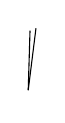
\begin{tikzpicture}[baseline=-.4ex,x=1ex,y=1ex]\draw (0,0) -- (.15,5);\draw (0,0) -- (.65,5.2);\end{tikzpicture}\,\uline{Mieux} Si $F''\ll F'\ll F\unsure{\in|\epsilon}$, \unsure{alors} $(F''\preccurlyeq F)\deleted{\unsure{\text{éq}|\Longrightarrow}}\Longleftrightarrow(F''\preccurlyeq F'\text{ et }F'\preccurlyeq F)$}

\uline{Proposition} \quad Considérons
\diagram{\begin{tikzcd}[ampersand replacement=\&,row sep=2pt,column sep=5pt]
F' \& \ll \& \deleted{\unsure{G}}F\\
\unsure{\rotatebox{90}{$\leqslant$}|\rotatebox{90}{$\leq$}} \& {} \& \rotatebox{90}{$\leqslant$}\\
\deleted{\unsure{G|E}}F'_G \& \ll \& G
\end{tikzcd}}
Si $F'\preccurlyeq F$, alors $F'_G\preccurlyeq G$.

En effet, \deleted{soit $K\in\mathcal F$, avec $x$} \inserted{il suffit de voir que \deleted{\unsure{l'il|l'on}}} $\deleted{\forall x\in\unsure{\operatorname{om}|\operatorname{omb}}}$ pour $x\in\operatorname{omb}(G)$, on a $x\mathrel{\overline{\parallel}}F'_G$. Mais si on avait $x\parallel F'_G$, on aurait $x\parallel F'$ par le lemme p.~\unsure{87|82}, \unsure{contrairemt|contrairement} à $F'\preccurlyeq F$, qed.

\uline{Corollaire 1} \quad Soit $F'\ll F$, et $F_i\leqslant F$ $(i\in I)$ tels que $\operatorname{Sup} F_i=F$. Soit $F'_i=F'\mid F_i$ le raffinement de $F_i$ induit. Alors $F'\preccurlyeq F$
\[
\text{\unsure{ssi}}\quad F'_i\preccurlyeq F_i\qquad\forall i\in I.
\]
